% Jonathan Forhan
% EG-316 Report -- Project 1

\documentclass[12pt]{article}

% title section
\title{EG-316 Project 1}
\author{Jonathan Forhan}
\date{ }

% packages
\usepackage[margin=0.5in]{geometry}
\usepackage{graphicx}
\usepackage{tocloft}
\usepackage{caption}
\usepackage{multicol}
\usepackage{pgfplots}
\usepackage[american]{circuitikz}
\usepackage{siunitx}

% mu
\sisetup{math-micro=\text{μ},text-micro=μ}

% add dots to table of contents
\renewcommand{\cftsecleader}{\cftdotfill{\cftdotsep}}

% no sci notation
% \pgfplotsset{scaled y ticks=false}
% \pgfplotsset{scaled x ticks=false}

% unbolden components
\ctikzset{bipoles/thickness=1}

%% start document
\begin{document}

% title page
\maketitle
\tableofcontents
\thispagestyle{empty}
\clearpage

%%%%%%%%%%%%%%%%%%%%%%%%%%%%%%%%%%%%%%%%%%%%%%%%%%%%%%%%%%%%%%%%%%%%%%%%%%%%%%%
%% analysis
\section{Analysis}

%%%%%%%%%%%%%%%%%%%%%%%%%%%%%%%%%%%%%%%
%% circuit A
\subsection{Circuit A}
\begin{figure}[ht]
	\begin{center}
		\begin{circuitikz}
			% left loop
			\draw
			(0,0) to[V, invert, l=$6$V, v_=$V_{A1}$, f<=$I_{A1}$]
			(0,3) to[R, l=$150\mathrm{k}\Omega$, v=$V_{A2}$, f>^=$I_{A2}$]
			(4,3) to[R, l=$470\mathrm{k}\Omega$, v=$V_{A3}$, f>^=$I_{A3}$]
			(4,0) -- (0,0);

			% a
			\draw
			(4,3) to[short, -o]
			(9,3) ++ (16pt,0) node[left] {a};

			% b
			\draw
			(4,0) to[short, -o, R, l=$560\mathrm{k}\Omega$, v=$V_{A4}$, f>^=$I_{A4}$]
			(9,0) ++ (16pt,0) node[left] {b};

			% ground
			\draw
			(2,0) to (2,-0.5) node[tlground] {};
		\end{circuitikz}
		\caption{Circuit A with no load}
	\end{center}
\end{figure}

\begin{multicols}{2}
	\begin{center}
		\subsection*{Voltage}
		\begin{tabular}{l}
			$V_{A1}=6\mathrm{V}$ \vspace{4pt}                                                    \\
			$V_{A2}=\frac{R_{A2}}{R_{A2}+R_{A3}}\left(V_{A1}\right)=1.45\mathrm{V}$ \vspace{4pt} \\
			$V_{A3}=\frac{R_{A3}}{R_{A2}+R_{A3}}\left(V_{A1}\right)=4.55\mathrm{V}$ \vspace{4pt} \\
			$V_{A4}=0\mathrm{V}$                                                                 \\
		\end{tabular}
		(1)
	\end{center}
	\begin{center}
		\subsection*{Current}
		\begin{tabular}{l}
			$I_{A1}=-I_{A2}=-9.67\textrm{\textmu}\mathrm{A}$ \vspace{4pt}              \\
			$I_{A2}=\frac{V_{A2}}{R_{A2}}=9.67\textrm{\textmu}\mathrm{A}$ \vspace{4pt} \\
			$I_{A3}=\frac{V_{A3}}{R_{A3}}=9.67\textrm{\textmu}\mathrm{A}$ \vspace{4pt} \\
			$I_{A4}=0\mathrm{A}$
		\end{tabular}
		(2)
	\end{center}
\end{multicols}

\clearpage

\subsection*{Th\'evenin-Norton}

% thevenin-norton step 1
\begin{figure}[ht]
	\begin{center}
		\begin{circuitikz}
			% loop
			\draw
			(0,3) to[I, invert, l_=$40$\textmu A]
			(0,0) to
			(3,0) to[R, l=$113\mathrm{k}\Omega$]
			(3,3);

			% a
			\draw
			(0,3) to[short, -o]
			(6,3) ++ (16pt,0) node[left] {a};

			% b
			\draw
			(3,0) to[short, -o, R, l=$560\mathrm{k}\Omega$]
			(6,0) ++ (16pt,0) node[left] {b};
		\end{circuitikz}
		\caption{Circuit A Norton intermediate step}
	\end{center}
\end{figure}

% thevenin-norton step 2
\begin{multicols}{2}
	\begin{center}
		\subsection*{Norton Equivalent}
		\begin{circuitikz}
			% loop
			\draw
			(0,0) to[I, l=$6.75$\textmu A]
			(0,3) to
			(3,3) to[R, l=$674\mathrm{k}\Omega$]
			(3,0);

			% a
			\draw
			(3,3) to[short, -o]
			(4,3) ++ (16pt,0) node[left] {a};

			% b
			\draw
			(0,0) to[short, -o]
			(4,0) ++ (16pt,0) node[left] {b};
		\end{circuitikz}
		\captionof{figure}{Circuit A Norton configuration}
	\end{center}
	\begin{center}
		\subsection*{Th\'evenin Equivalent}
		\begin{circuitikz}
			% loop
			\draw
			(0,0) to[V, invert, l=$4.55$V]
			(0,3) to[R, l=$674\mathrm{k}\Omega$]
			(4,3);

			% a
			\draw
			(4,3) to[short, -o]
			(4,3) ++ (16pt,0) node[left] {a};

			% b
			\draw
			(0,0) to[short, -o]
			(4,0) ++ (16pt,0) node[left] {b};
		\end{circuitikz}
		\captionof{figure}{Circuit A Th\'evenin configuration}
	\end{center}
\end{multicols}

\subsection*{Maximum load power}

The maximum power transfer theorem for DC circuits states that, when the load resistance $R_L$ equals the Th\'evenin equivalent resistance across $R_L$, maximum power is transferred to the load.
The maximum power transfer theorem also tells us that when $R_L$ equals $R_{\textrm{Th}}$, $P_{\mathrm{max}}=\frac{V^2}{4R_{L}}$, thus for maximum power transfer:

$$R_L=674\mathrm{k}\Omega$$
$$P_{\mathrm{max}}=7.68\textrm{\textmu}\mathrm{W}$$

\begin{center}
	(3)
\end{center}

\clearpage


%%%%%%%%%%%%%%%%%%%%%%%%%%%%%%%%%%%%%%%
%% circuit B
\subsection{Circuit B}
\begin{figure}[ht]
	\begin{center}
		\begin{circuitikz}
			% left loop
			\draw
			(0,0) to[V, invert, l=$6$V, v_=$V_{B1}$, f<=$I_{B1}$]
			(0,3) to[R, l=$15\mathrm{k}\Omega$, v=$V_{B2}$, f>^=$I_{B2}$]
			(4,3) to[R, l=$47\mathrm{k}\Omega$, v=$V_{B3}$, f>=$I_{B3}$]
			(4,0) -- (0,0);

			% right loop
			\draw
			(4,3) to[R, l=$56\mathrm{k}\Omega$, v=$V_{B4}$, f>^=$I_{B4}$]
			(8,3) to[R, l=$56\mathrm{k}\Omega$, v=$V_{B5}$, f>^=$I_{B5}$]
			(8,0) -- (4,0);

			% a
			\draw
			(8,3) to[short, -o]
			(9,3) ++ (16pt,0) node[left] {a};

			% b
			\draw
			(8,0) to[short, -o]
			(9,0) ++ (16pt,0) node[left] {b};

			% ground
			\draw
			(2,0) to (2,-0.5) node[tlground] {};
		\end{circuitikz}
		\caption{Circuit B with no load}
	\end{center}
\end{figure}

\begin{center}
	\[ R_{\mathrm{eq}}=\frac{\left(R_{B4}+R_{B5}\right)R_{B3}}{R_{B3}+R_{B4}+R_{B5}}+R_{B2}=48.1\mathrm{k}\Omega \]
	\[ I_{\mathrm{eq}}=\frac{V_{B1}}{R_{\mathrm{eq}}}=125\textrm{\textmu}\mathrm{A} \]
\end{center}

\begin{multicols}{2}
	\begin{center}
		\subsection*{Voltage}
		\begin{tabular}{l}
			$V_{B1}=\mathrm{6V}$ \vspace{4pt}                        \\
			$V_{B2}=I_{B2}\times R_{B2}=1.87\mathrm{V}$ \vspace{4pt} \\
			$V_{B3}=V_{B1}-V_{B2}=4.13\mathrm{V}$ \vspace{4pt}       \\
			$V_{B4}=I_{B4}\times R_{B4}=2.08\mathrm{V}$ \vspace{4pt} \\
			$V_{B5}=V_{B3}-V_{B4}=2.05\mathrm{V}$
		\end{tabular}
		(4)
	\end{center}
	\begin{center}
		\subsection*{Current}
		\begin{tabular}{l}
			$I_{B1}=-I_{\mathrm{eq}}=-125\textrm{\textmu A}$ \vspace{4pt}      \\
			$I_{B2}=I_{\mathrm{eq}}=125\textrm{\textmu A}$ \vspace{4pt}        \\
			$I_{B3}=\frac{V_{B3}}{R_{B3}}=87.9\textrm{\textmu A}$ \vspace{4pt} \\
			$I_{B4}=I_{B2}-I_{B3}=37.1\textrm{\textmu A}$ \vspace{4pt}         \\
			$I_{B5}=I_{B4}=37.1\textrm{\textmu A}$
		\end{tabular}
		(5)
	\end{center}
\end{multicols}

\clearpage

\subsection*{Th\'evenin-Norton}

% thevenin-norton step 1
\begin{multicols}{2}
	\begin{center}
		\begin{circuitikz}
			% loop
			\draw
			(0,3) to[I, invert, l_=$400$\textmu A]
			(0,0) to
			(3,0) to[R, l=$11.4\mathrm{k}\Omega$]
			(3,3);

			% right-loop
			\draw
			(0,3) to
			(3,3) to[R, l=$56\mathrm{k}\Omega$]
			(6,3) to[R, l=$56\mathrm{k}\Omega$]
			(6,0) -- (3,0);

			% a
			\draw
			(6,3) to[short, -o]
			(7,3) ++ (16pt,0) node[left] {a};

			% b
			\draw
			(6,0) to[short, -o]
			(7,0) ++ (16pt,0) node[left] {b};
		\end{circuitikz}
		\captionof{figure}{Circuit B Norton intermediate step}
	\end{center}
	\begin{center}
		\begin{circuitikz}
			% loop
			\draw
			(0,0) to[V, invert, l_=$4.54$V]
			(0,3) to[R, l=$67.4\mathrm{k}\Omega$]
			(3,3) to[R, l=$56\mathrm{k}\Omega$]
			(3,0) -- (0,0);

			% a
			\draw
			(3,3) to[short, -o]
			(4,3) ++ (16pt,0) node[left] {a};

			% b
			\draw
			(3,0) to[short, -o]
			(4,0) ++ (16pt,0) node[left] {b};
		\end{circuitikz}
		\captionof{figure}{Circuit B Th\'evenin intermediate step}
	\end{center}
\end{multicols}

\vspace{1em}

% thevenin-norton step 3
\begin{multicols}{2}
	\begin{center}
		\subsection*{Norton Equivalent}
		\begin{circuitikz}
			% loop
			\draw
			(0,0) to[I, l_=$67.7\textrm{\textmu A}$]
			(0,3) to
			(3,3) to[R, l=$30.6\mathrm{k}\Omega$]
			(3,0) -- (0,0);

			% a
			\draw
			(3,3) to[short, -o]
			(4,3) ++ (16pt,0) node[left] {a};

			% b
			\draw
			(3,0) to[short, -o]
			(4,0) ++ (16pt,0) node[left] {b};
		\end{circuitikz}
		\captionof{figure}{Circuit B Norton equivalent}
	\end{center}
	\begin{center}
		\subsection*{Th\'evenin Equivalent}
		\begin{circuitikz}
			% loop
			\draw
			(0,0) to[V, invert, l_=$2.07$V]
			(0,3) to[R, l=$30.6\mathrm{k}\Omega$]
			(3,3) to[short, -o] % a
			(3,3) ++ (16pt,0) node[left] {a};

			% b
			\draw
			(0,0) to[short, -o]
			(3,0) ++ (16pt,0) node[left] {b};
		\end{circuitikz}
		\captionof{figure}{Circuit B Th\'evenin equivalent}
	\end{center}
\end{multicols}

\subsection*{Maximum load power}

As stated in circuit A's \textit{Maximum load power} section,
the maximum power transfer theorem tells us that $R_L$ equals $R_{\textrm{Th}}$ and $P_{\mathrm{max}}=\frac{V^2}{4R_{L}}$, thus for maximum power transfer:

$$R_L=30.6\mathrm{k}\Omega$$
$$P_{\mathrm{max}}=35.0\textrm{\textmu}\mathrm{W}$$

\begin{center}
	(6)
\end{center}

\clearpage

\section{Simulation}

\subsection{Circuit A}

\begin{center}
	\begin{multicols}{2}
		\begin{center}
			\begin{tabular}{c|c}
				$V_{A1}$ & 6V    \\
				$V_{A2}$ & 1.45V \\
				$V_{A3}$ & 4.55V \\
				$V_{A4}$ & 0V    \\
			\end{tabular}
			\captionof{table}{Circuit A simulated voltages}
		\end{center}
		\begin{center}
			\begin{tabular}{c|c}
				$I_{A1}$ & -9.68\textmu A \\
				$I_{A2}$ & 9.68\textmu A  \\
				$I_{A3}$ & 9.68\textmu A  \\
				$I_{A4}$ & 0\textmu A     \\
			\end{tabular}
			\captionof{table}{Circuit A simulated currents}
		\end{center}
	\end{multicols}
\end{center}

\subsection*{Sweep}

\begin{figure}[h]
	\begin{center}
		\begin{tikzpicture}
			\begin{axis}[
					width=16cm,
					height=8cm,
					xlabel=Load Resistance $R_L$,
					ylabel=Power $W_L$,
					ymax=7.69E-06,
					grid=both,
					y tick label style={scaled y ticks=base 10:6},
					x tick label style={scaled x ticks=base 10:-3}
				]
				\addplot[ultra thick,black] table [mark=none,x=X,y=Y,col sep=comma]{res/Circuit_A_sweep_600k-750k.csv};
				\addplot [ultra thick,black,only marks] table {
						672483 0.00000767683
					};
				\node[black] at (73.6,30.6) {$R_L=672.483\mathrm{k}\Omega$, $W_L=7.67683\textrm{\textmu W}$};
			\end{axis}
		\end{tikzpicture}
		\caption{Circuit A sweep, $R_L$ versus $W_L$}
	\end{center}
\end{figure}

Figure 10 corresponds with the analysis values for the load resistance and power of $674$k$\Omega$ and $7.68$\textmu W.

\clearpage

\subsection{Circuit B}

\begin{center}
	\begin{multicols}{2}
		\begin{center}
			\begin{tabular}{c|c}
				$V_{A1}$ & 6V    \\
				$V_{A2}$ & 1.87V \\
				$V_{A3}$ & 4.13V \\
				$V_{A4}$ & 2.06V \\
				$V_{A5}$ & 2.06V \\
			\end{tabular}
			\captionof{table}{Circuit B simulated voltages}
		\end{center}
		\begin{center}
			\begin{tabular}{c|c}
				$I_{A1}$ & -125\textmu A \\
				$I_{A2}$ & 125\textmu A  \\
				$I_{A3}$ & 89.9\textmu A \\
				$I_{A4}$ & 36.9\textmu A \\
				$I_{A5}$ & 36.9\textmu A \\
			\end{tabular}
			\captionof{table}{Circuit B simulated currents}
		\end{center}
	\end{multicols}
\end{center}

\subsection*{Sweep}

\begin{figure}[h]
	\begin{center}
		\begin{tikzpicture}
			\begin{axis}[
					width=16cm,
					height=8cm,
					xlabel=Load Resistance $R_L$,
					ylabel=Power $W_L$,
					ymax=35.5E-6,
					grid=both,
					y tick label style={scaled y ticks=base 10:6},
					x tick label style={scaled x ticks=base 10:-3}
				]
				\addplot [ultra thick,black] table [mark=none,x=X,y=Y,col sep=comma]{res/Circuit_B_sweep_20k-50k.csv};
				\addplot [ultra thick,black,only marks] table {
						30671.14 0.000034846
					};
				\node[black] at (120,230) {$R_L=30.67\mathrm{k}\Omega$, $W_L=34.846\textrm{\textmu W}$};
			\end{axis}
		\end{tikzpicture}
		\caption{Circuit A sweep, $R_L$ versus $W_L$}
	\end{center}
\end{figure}

Figure 11 corresponds with the analysis values for the load resistance and power of $30.7$k$\Omega$ and $34.8$\textmu W.

\clearpage

\section{Measurement}

\subsection{Circuit A}

\begin{center}
	\begin{multicols}{2}
		\begin{center}
			\begin{tabular}{c|c}
				$V_{A1}$ & 6.06V \\
				$V_{A2}$ & 1.32V \\
				$V_{A3}$ & 4.12V \\
				$V_{A4}$ & 0V    \\
			\end{tabular}
			\captionof{table}{Circuit A measured voltages}
		\end{center}
		\begin{center}
			\begin{tabular}{c|c}
				$I_{A1}$ & -9.7\textmu A \\
				$I_{A2}$ & 9.7\textmu A  \\
				$I_{A3}$ & 9.9\textmu A  \\
				$I_{A4}$ & 0\textmu A    \\
			\end{tabular}
			\captionof{table}{Circuit A measured currents}
		\end{center}
	\end{multicols}
\end{center}

\subsection*{Testing load power}

Resistances used: 600k, 625k, 650k, 675k, 700k.

\begin{center}
	\begin{tabular}{|c|c|c|}
		\hline
		Measured Resistance               & Measured Current      & Power                  \\
		\hline
		$616$k$\Omega$                    & 3.5\textmu A          & 7.55\textmu W          \\
		$641$k$\Omega$                    & 3.4\textmu A          & 7.41\textmu W          \\
		\textbf{\boldmath $666$k$\Omega$} & \textbf{3.4\textmu A} & \textbf{7.70\textmu W} \\
		$692$k$\Omega$                    & 3.3\textmu A          & 7.54\textmu W          \\
		$716$k$\Omega$                    & 3.2\textmu A          & 7.33\textmu W          \\
		\hline
	\end{tabular}
	\captionof{table}{Circuit A raw load power measurements}
\end{center}

\begin{figure}[h]
	\centering
	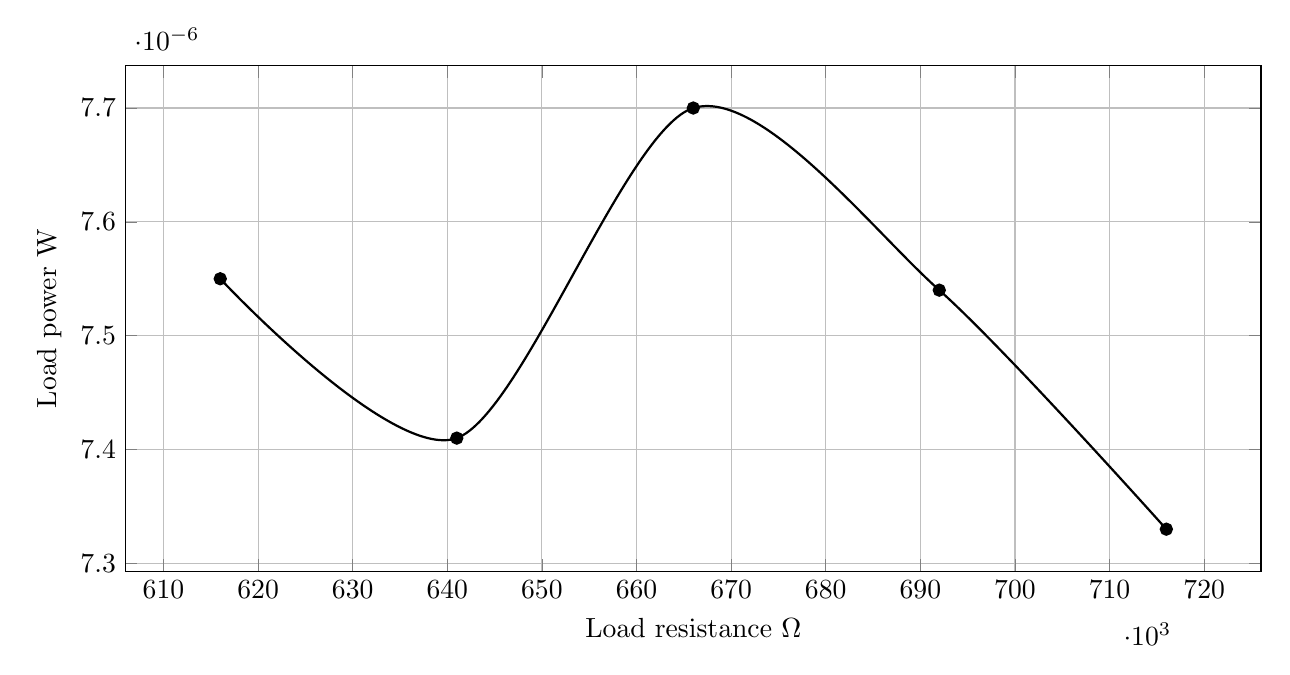
\begin{tikzpicture}
		\begin{axis}[
				width=16cm,
				height=8cm,
				xlabel=Load resistance $\Omega$,
				ylabel=Load power W,
				grid=both,
				y tick label style={scaled y ticks=base 10:6},
				x tick label style={scaled x ticks=base 10:-3}
			]
			\addplot[thick,smooth,mark=*,black] plot coordinates {
					(616000,0.00000755)
					(641000,0.00000741)
					(666000,0.00000770)
					(692000,0.00000754)
					(716000,0.00000733)
				};
		\end{axis}
	\end{tikzpicture}
	\caption{Circuit A load resistance plotted against load power}
\end{figure}

\clearpage

\subsection{Circuit B}

\begin{center}
	\begin{multicols}{2}
		\begin{center}
			\begin{tabular}{c|c}
				$V_{A1}$ & 6.06V \\
				$V_{A2}$ & 1.87V \\
				$V_{A3}$ & 4.12V \\
				$V_{A4}$ & 2.01V \\
				$V_{A5}$ & 2.01V \\
			\end{tabular}
			\captionof{table}{Circuit B measured voltages}
		\end{center}
		\begin{center}
			\begin{tabular}{c|c}
				$I_{A1}$ & -123\textmu A \\
				$I_{A2}$ & 123\textmu A  \\
				$I_{A3}$ & 91.8\textmu A \\
				$I_{A4}$ & 37.0\textmu A \\
				$I_{A5}$ & 36.8\textmu A \\
			\end{tabular}
			\captionof{table}{Circuit B measured currents}
		\end{center}
	\end{multicols}
\end{center}

\subsection*{Testing load power}

Resistances used: 20k, 25k, 30k, 35k, 40k.

\begin{center}
	\begin{tabular}{|c|c|c|}
		\hline
		Measured Resistance                & Measured Current       & Power                  \\
		\hline
		$19.7$k$\Omega$                    & 40.2\textmu A          & 31.9\textmu W          \\
		$24.8$k$\Omega$                    & 36.7\textmu A          & 33.4\textmu W          \\
		$29.6$k$\Omega$                    & 33.8\textmu A          & 33.8\textmu W          \\
		\textbf{\boldmath $34.7$k$\Omega$} & \textbf{31.3\textmu A} & \textbf{34.0\textmu W} \\
		$39.6$k$\Omega$                    & 29.1\textmu A          & 33.5\textmu W          \\
		\hline
	\end{tabular}
	\captionof{table}{Circuit B raw load power measurements}
\end{center}

\begin{figure}[h]
	\centering
	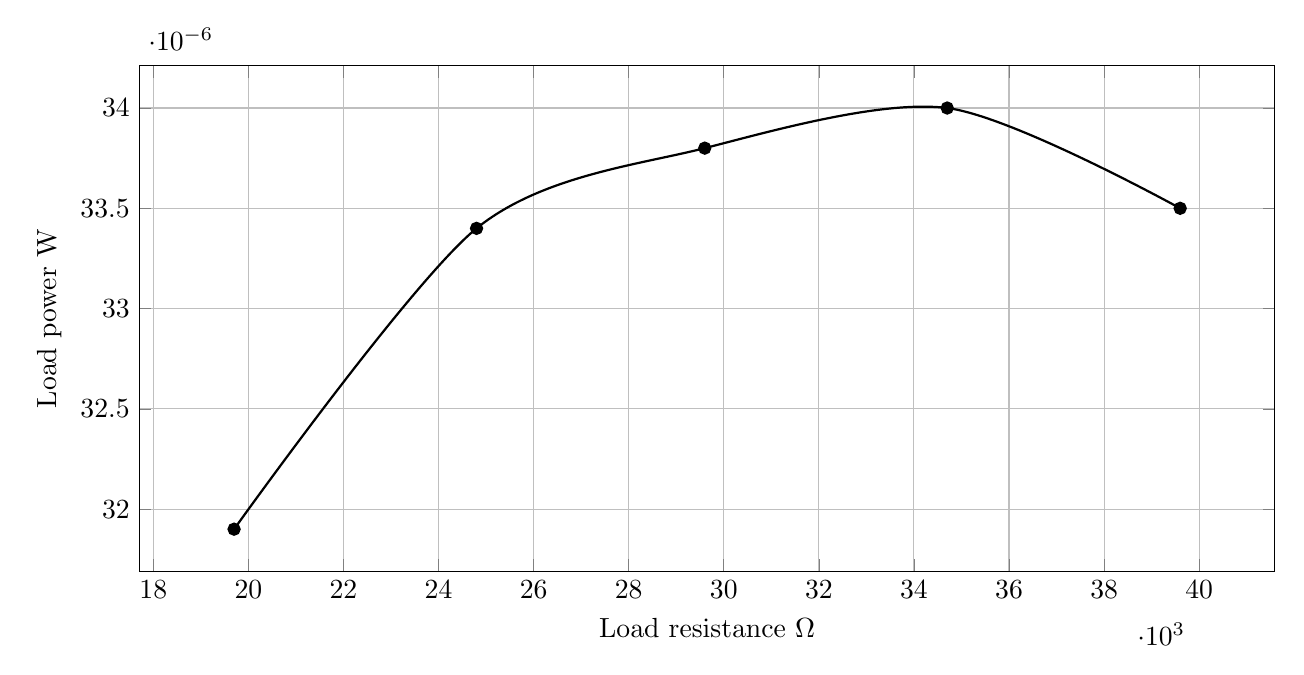
\begin{tikzpicture}
		\begin{axis}[
				width=16cm,
				height=8cm,
				xlabel=Load resistance $\Omega$,
				ylabel=Load power W,
				grid=both,
				y tick label style={scaled y ticks=base 10:6},
				x tick label style={scaled x ticks=base 10:-3}
			]
			\addplot[thick,smooth,mark=*,black] plot coordinates {
					(19700,0.0000319)
					(24800,0.0000334)
					(29600,0.0000338)
					(34700,0.0000340)
					(39600,0.0000335)
				};
		\end{axis}
	\end{tikzpicture}
	\caption{Circuit B load resistance plotted against load power}
\end{figure}


\clearpage

\section{Model discrepancies}

\subsection{Data comparison}


\begin{center}
	\begin{tabular}{|c|c|c|c|}
		\hline
		         & Analysis       & Simulation     & Measured      \\
		\hline
		$V_{A1}$ & 6V             & 6V             & 6.06V         \\
		$I_{A1}$ & -9.67\textmu A & -9.68\textmu A & -9.7\textmu A \\
		\hline
		$V_{A2}$ & 1.45V          & 1.45V          & 1.32V         \\
		$I_{A2}$ & 9.67\textmu A  & 9.68\textmu A  & 9.7\textmu A  \\
		\hline
		$V_{A3}$ & 4.55V          & 4.55V          & 4.12V         \\
		$I_{A3}$ & 9.67\textmu A  & 9.68\textmu A  & 9.9\textmu A  \\
		\hline
		$V_{A4}$ & 0V             & 0V             & 0V            \\
		$I_{A4}$ & 0A             & 0A             & 0A            \\
		\hline
		$R_{AL}$ & 674k$\Omega$   & 673k$\Omega$   & 666k$\Omega$  \\
		$W_{AL}$ & 7.68\textmu W  & 7.68\textmu W  & 7.70\textmu W \\
		\hline
		\hline
		$V_{B1}$ & 6V             & 6V             & 6.06V         \\
		$I_{B1}$ & -125\textmu A  & -125\textmu A  & -123\textmu A \\
		\hline
		$V_{B2}$ & 1.87V          & 1.87V          & 1.87V         \\
		$I_{B2}$ & 125\textmu A   & 125\textmu A   & 123\textmu A  \\
		\hline
		$V_{B3}$ & 4.13V          & 4.13V          & 4.12V         \\
		$I_{B3}$ & 87.9\textmu A  & 89.9\textmu A  & 91.8\textmu A \\
		\hline
		$V_{B4}$ & 2.08V          & 2.06V          & 2.01V         \\
		$I_{B4}$ & 37.1\textmu A  & 36.9\textmu A  & 37.0\textmu A \\
		\hline
		$V_{B5}$ & 2.05V          & 2.06V          & 2.01V         \\
		$I_{B5}$ & 37.1\textmu A  & 36.9\textmu A  & 36.8\textmu A \\
		\hline
		$R_{BL}$ & 30.6k$\Omega$  & 30.7k$\Omega$  & 34.7k$\Omega$ \\
		$W_{BL}$ & 35.0\textmu W  & 34.8\textmu W  & 34.0\textmu W \\
		\hline
	\end{tabular}
	\captionof{table}{Comparison of element values across analysis, simulation, and measurements.}
\end{center}

\clearpage

Resistances used: 616k$\Omega$, 641k$\Omega$, 666k$\Omega$, 692k$\Omega$, 716k$\Omega$.
\begin{figure}[h]
	\centering
	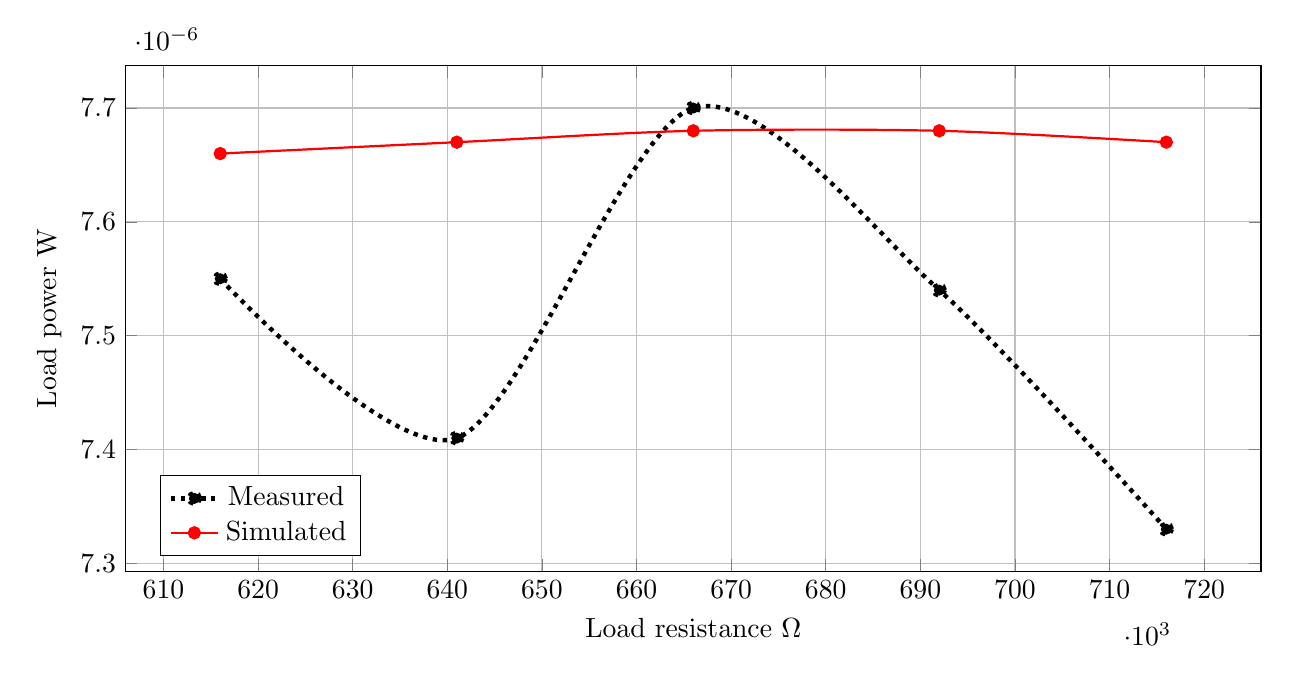
\begin{tikzpicture}
		\begin{axis}[
				width=16cm,
				height=8cm,
				xlabel=Load resistance $\Omega$,
				ylabel=Load power W,
				grid=both,
				y tick label style={scaled y ticks=base 10:6},
				x tick label style={scaled x ticks=base 10:-3},
				legend pos=south west
			]
			\addplot[ultra thick,smooth,mark=*,black,dotted] plot coordinates {
					(616000,0.00000755)
					(641000,0.00000741)
					(666000,0.00000770)
					(692000,0.00000754)
					(716000,0.00000733)
				};
			\addplot[thick,smooth,mark=*,red] plot coordinates {
					(616000,0.00000766)
					(641000,0.00000767)
					(666000,0.00000768)
					(692000,0.00000768)
					(716000,0.00000767)
				};
			\addlegendentry{Measured}
			\addlegendentry{Simulated}
		\end{axis}
	\end{tikzpicture}
	\caption{Circuit A load resistance plotted against load power}
\end{figure}

\vspace{1em}

Resistances used: 19.7k$\Omega$, 24.8k$\Omega$, 29.6k$\Omega$, 34.7k$\Omega$, 39.6k$\Omega$.

\begin{figure}[h]
	\centering
	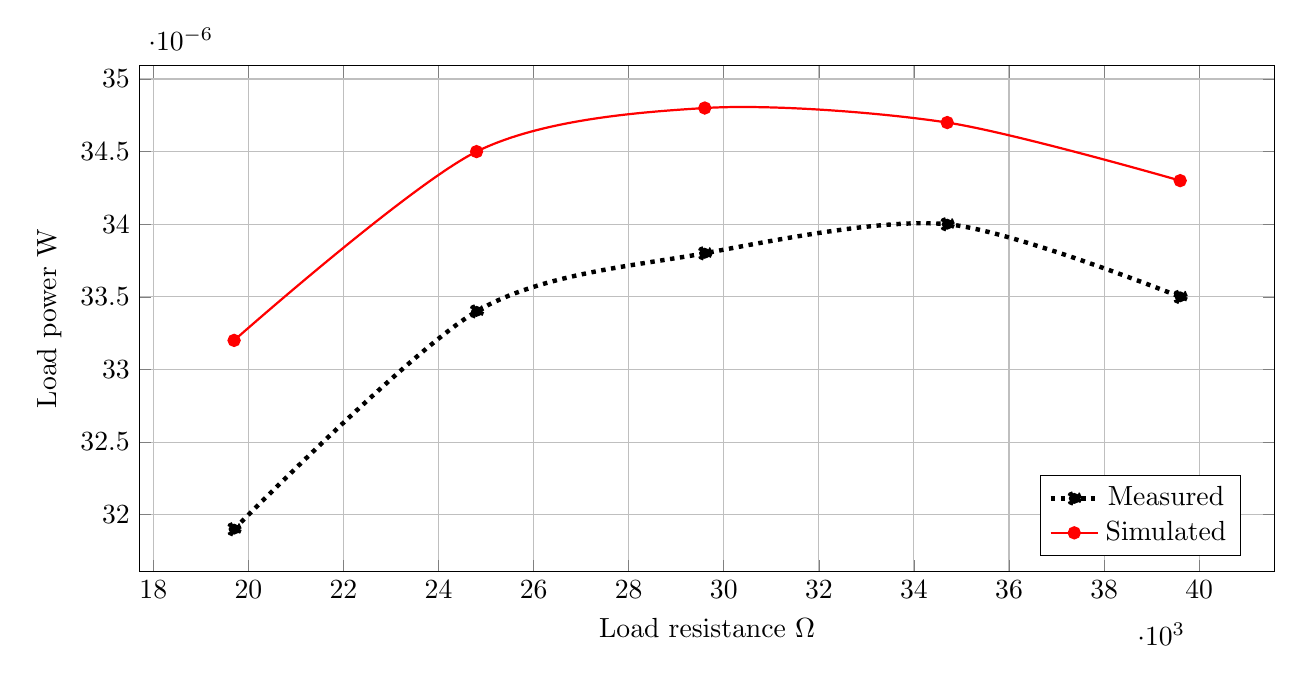
\begin{tikzpicture}
		\begin{axis}[
				width=16cm,
				height=8cm,
				xlabel=Load resistance $\Omega$,
				ylabel=Load power W,
				grid=both,
				y tick label style={scaled y ticks=base 10:6},
				x tick label style={scaled x ticks=base 10:-3},
				legend pos=south east
			]
			\addplot[ultra thick,smooth,mark=*,black,dotted] plot coordinates {
					(19700,0.0000319)
					(24800,0.0000334)
					(29600,0.0000338)
					(34700,0.0000340)
					(39600,0.0000335)
				};
			\addplot[thick,smooth,mark=*,red] plot coordinates {
					(19700,0.0000332)
					(24800,0.0000345)
					(29600,0.0000348)
					(34700,0.0000347)
					(39600,0.0000343)
				};
			\addlegendentry{Measured}
			\addlegendentry{Simulated}
		\end{axis}
	\end{tikzpicture}
	\caption{Circuit B load resistance plotted against load power}
\end{figure}

\subsection{Solution to the difference}

One source of difference that is affecting the measured results is the variance of resistance in the components.
A way to combat this is the measure the true resistance of the components and do our simulations around these values.
In the next section I will use the measured resistances to get a more accurate simulation.

\clearpage

\section{Improved Simulation}

\subsection{Improved values}

\begin{multicols}{2}
	\begin{center}
		\begin{tabular}{c|c}
			$R_{A2}$ & 148k$\Omega$ \\
			$R_{A3}$ & 460k$\Omega$ \\
			$R_{A4}$ & 553k$\Omega$ \\
		\end{tabular}
	\end{center}
	\begin{center}
		\begin{tabular}{c|c}
			$R_{B2}$ & 14.6k$\Omega$ \\
			$R_{B3}$ & 46.6k$\Omega$ \\
			$R_{B4}$ & 55.6k$\Omega$ \\
			$R_{B5}$ & 56.1k$\Omega$ \\
		\end{tabular}
	\end{center}
\end{multicols}
\captionof{table}{True values of the resistances used in the measured circuit}

\begin{center}
	\begin{tabular}{|c|c|c|c|c|}
		\hline
		         & Analysis       & Simulation     & Measured      & Improved Sim  \\
		\hline
		$V_{A1}$ & 6V             & 6V             & 6.06V         & 6V            \\
		$I_{A1}$ & -9.67\textmu A & -9.68\textmu A & -9.7\textmu A & -9.8\textmu A \\
		\hline
		$V_{A2}$ & 1.45V          & 1.45V          & 1.32V         & 1.44V         \\
		$I_{A2}$ & 9.67\textmu A  & 9.68\textmu A  & 9.7\textmu A  & 9.8\textmu A  \\
		\hline
		$V_{A3}$ & 4.55V          & 4.55V          & 4.12V         & 4.53V         \\
		$I_{A3}$ & 9.67\textmu A  & 9.68\textmu A  & 9.9\textmu A  & 9.8\textmu A  \\
		\hline
		$V_{A4}$ & 0V             & 0V             & 0V            & 0V            \\
		$I_{A4}$ & 0A             & 0A             & 0A            & 0A            \\
		\hline
		$R_{AL}$ & 674k$\Omega$   & 673k$\Omega$   & 666k$\Omega$  & 673k$\Omega$  \\
		$W_{AL}$ & 7.68\textmu W  & 7.68\textmu W  & 7.70\textmu W & 7.69\textmu W \\
		\hline
		\hline
		$V_{B1}$ & 6V             & 6V             & 6.06V         & 6V            \\
		$I_{B1}$ & -125\textmu A  & -125\textmu A  & -123\textmu A & -126\textmu A \\
		\hline
		$V_{B2}$ & 1.87V          & 1.87V          & 1.87V         & 1.87V         \\
		$I_{B2}$ & 125\textmu A   & 125\textmu A   & 123\textmu A  & 126\textmu A  \\
		\hline
		$V_{B3}$ & 4.13V          & 4.13V          & 4.12V         & 4.14V         \\
		$I_{B3}$ & 87.9\textmu A  & 89.9\textmu A  & 91.8\textmu A & 90.0\textmu A \\
		\hline
		$V_{B4}$ & 2.08V          & 2.06V          & 2.01V         & 2.05V         \\
		$I_{B4}$ & 37.1\textmu A  & 36.9\textmu A  & 37.0\textmu A & 37.2\textmu A \\
		\hline
		$V_{B5}$ & 2.05V          & 2.06V          & 2.01V         & 2.05V         \\
		$I_{B5}$ & 37.1\textmu A  & 36.9\textmu A  & 36.8\textmu A & 37.2\textmu A \\
		\hline
		$R_{BL}$ & 30.6k$\Omega$  & 30.7k$\Omega$  & 34.7k$\Omega$ & 30.9k$\Omega$ \\
		$W_{BL}$ & 35.0\textmu W  & 34.8\textmu W  & 34.0\textmu W & 34.7\textmu W \\
		\hline
	\end{tabular}
	\captionof{table}{Comparison of element values, now including improved simulation.}
\end{center}

The gains here are small because the analysis, simulation, and measurements aligned very well already.

\section{Photos}

\begin{center}
	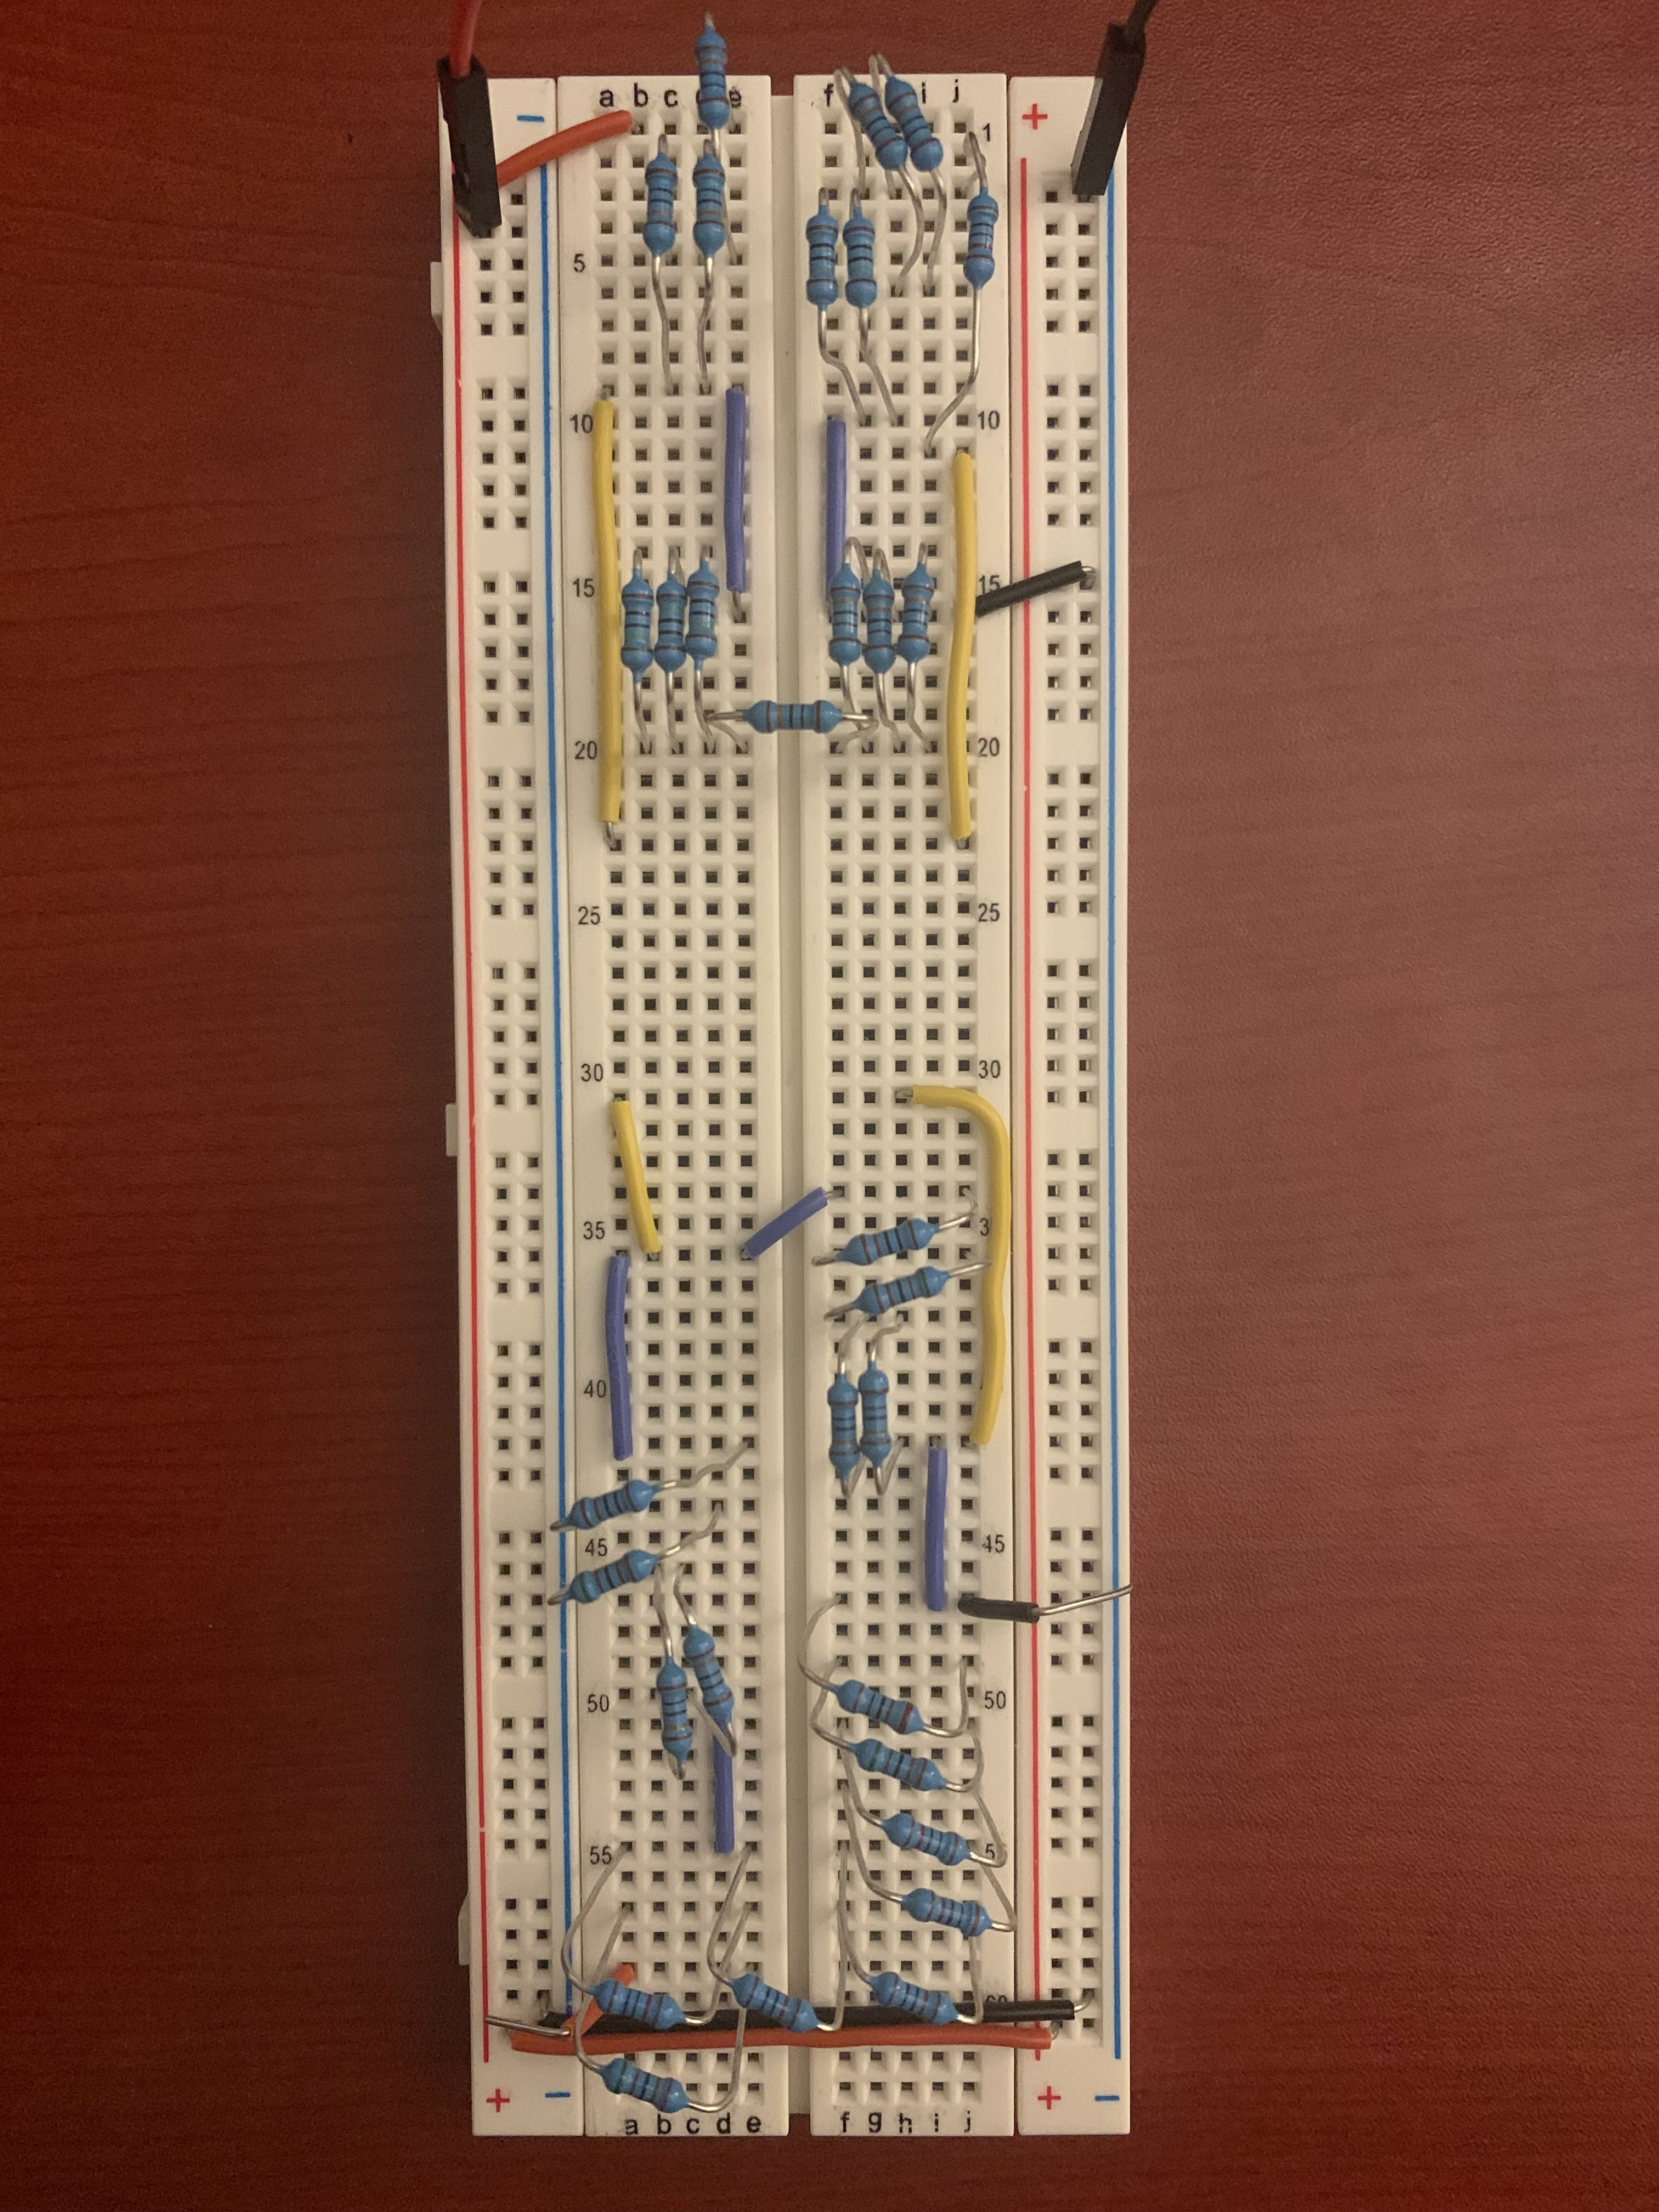
\includegraphics[width=0.9\textwidth]{res/IMG_0149.jpg}
	\newline
	Circuit A on top, cirbuit B on bottom
\end{center}

\clearpage

\begin{center}
	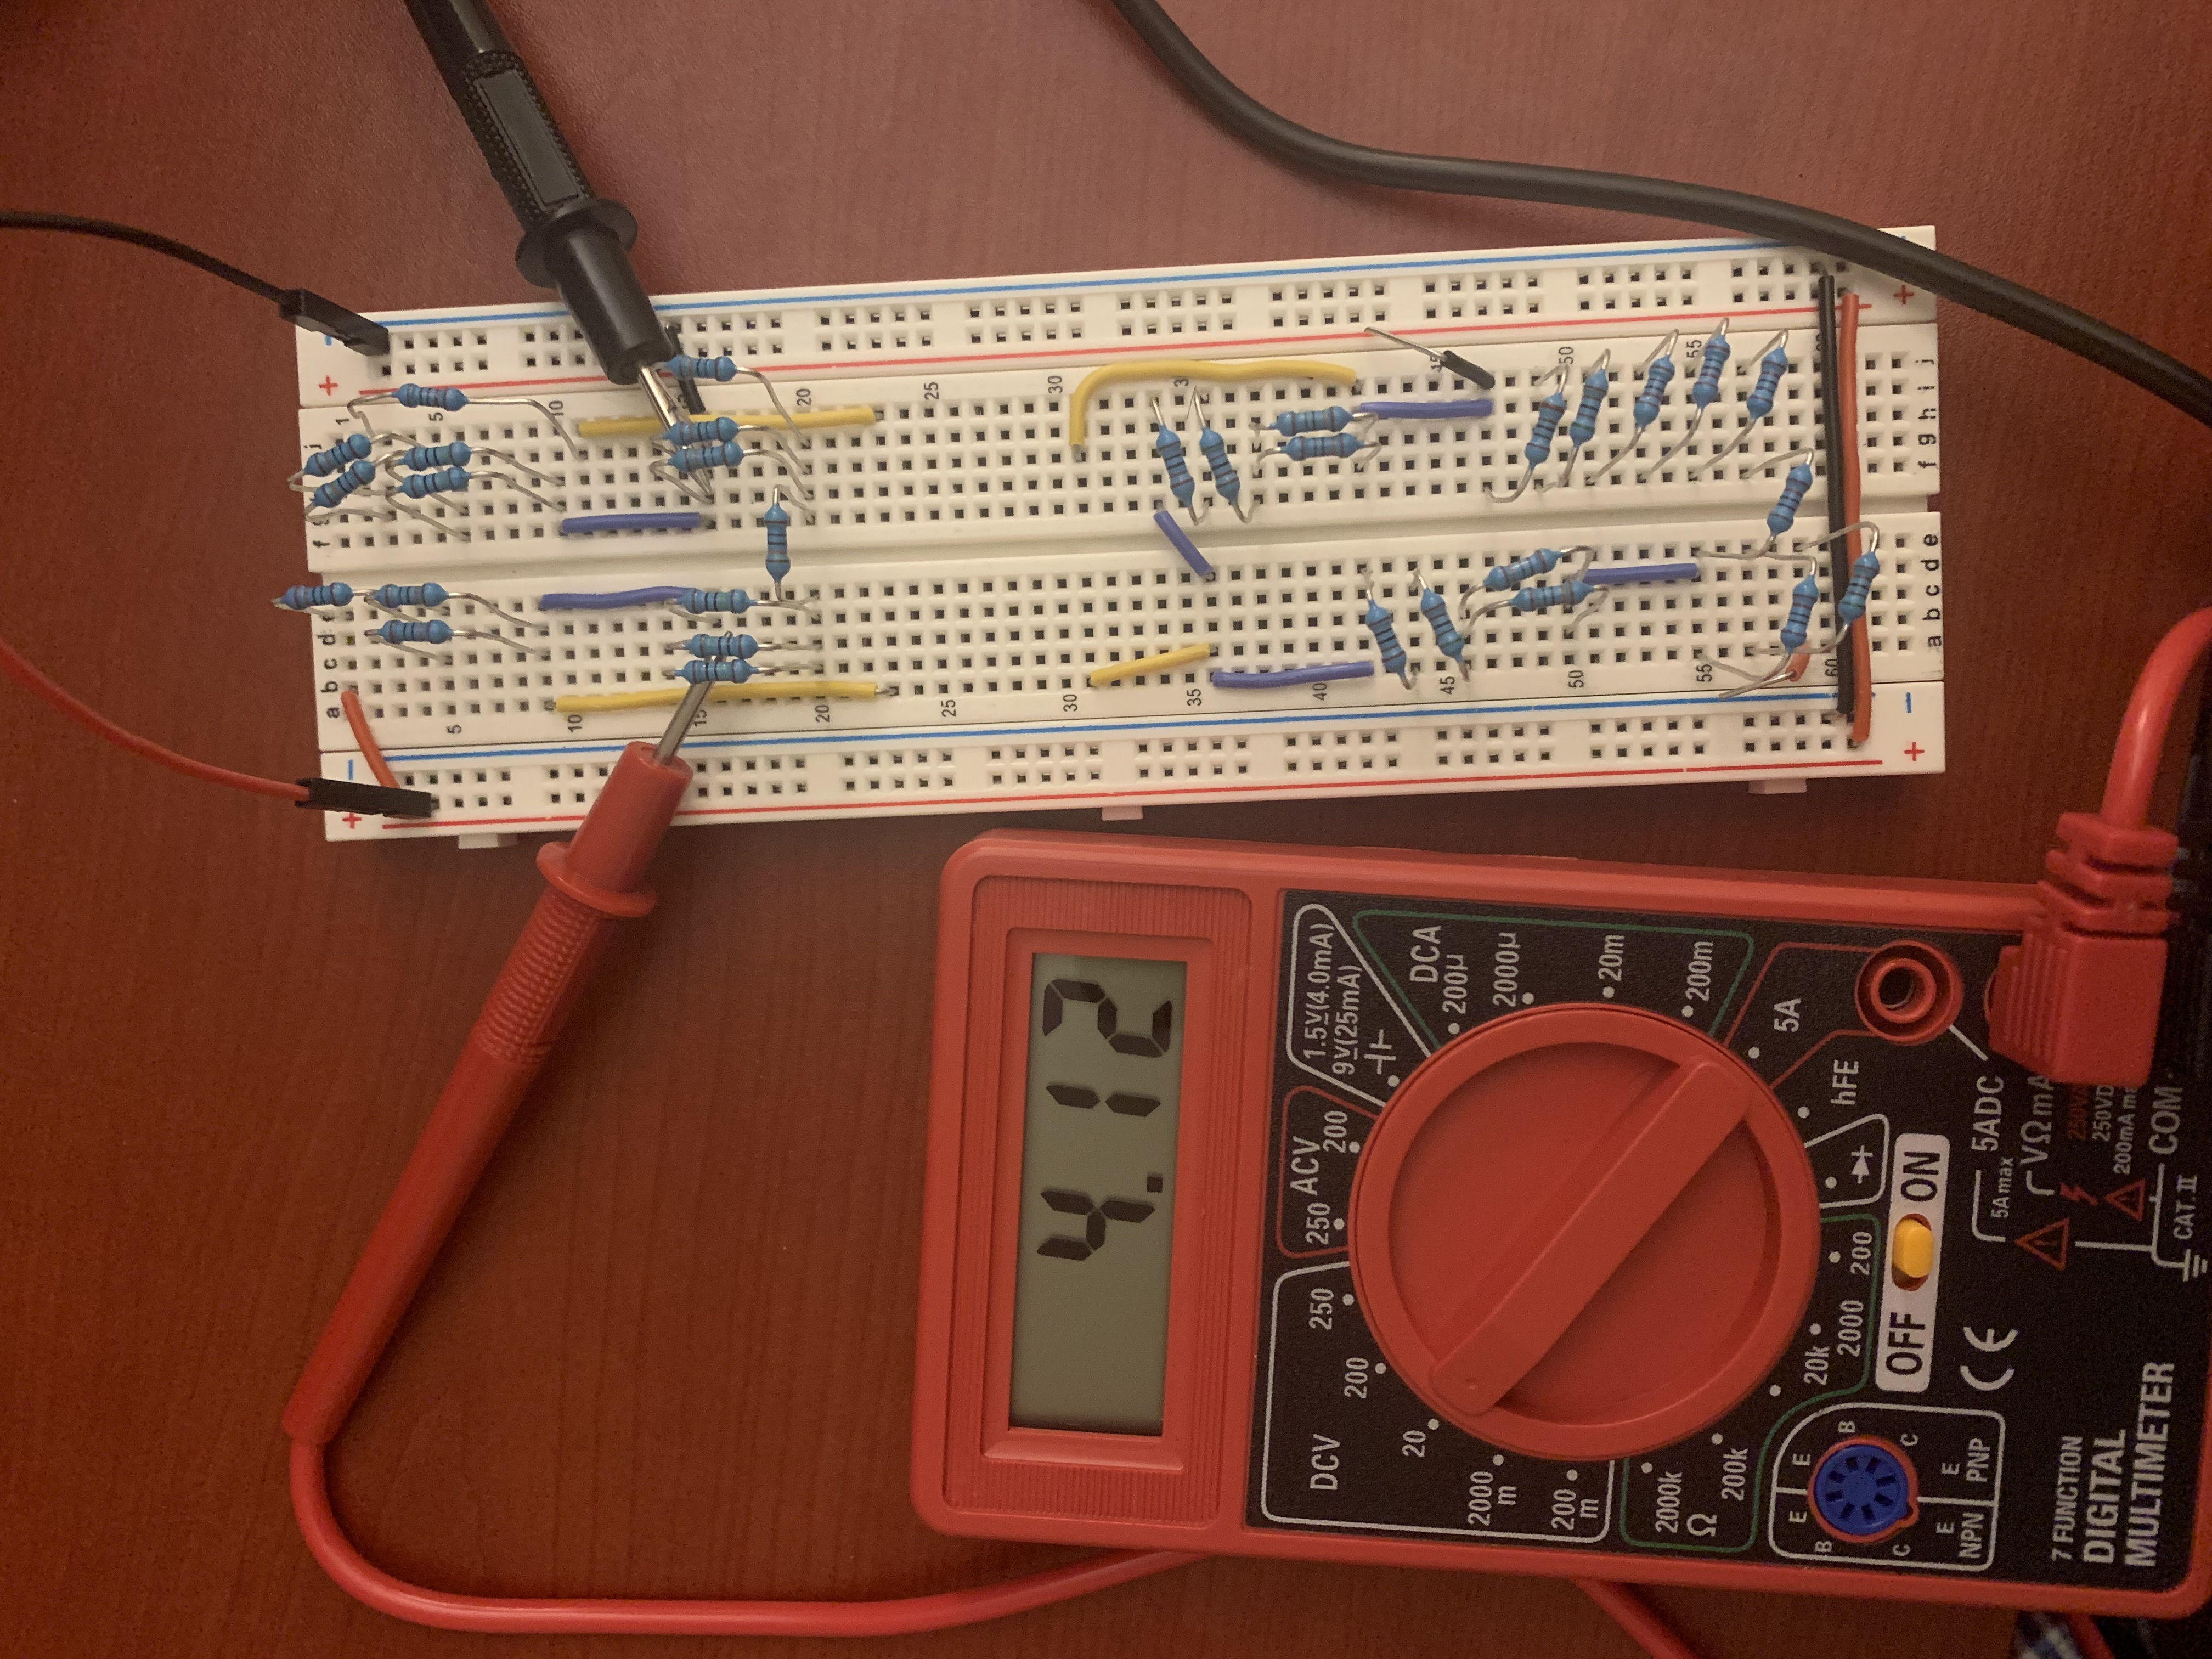
\includegraphics[width=0.8\textwidth]{res/IMG_0150.jpg}
	\newline
	Measuring voltage
\end{center}
\begin{center}
	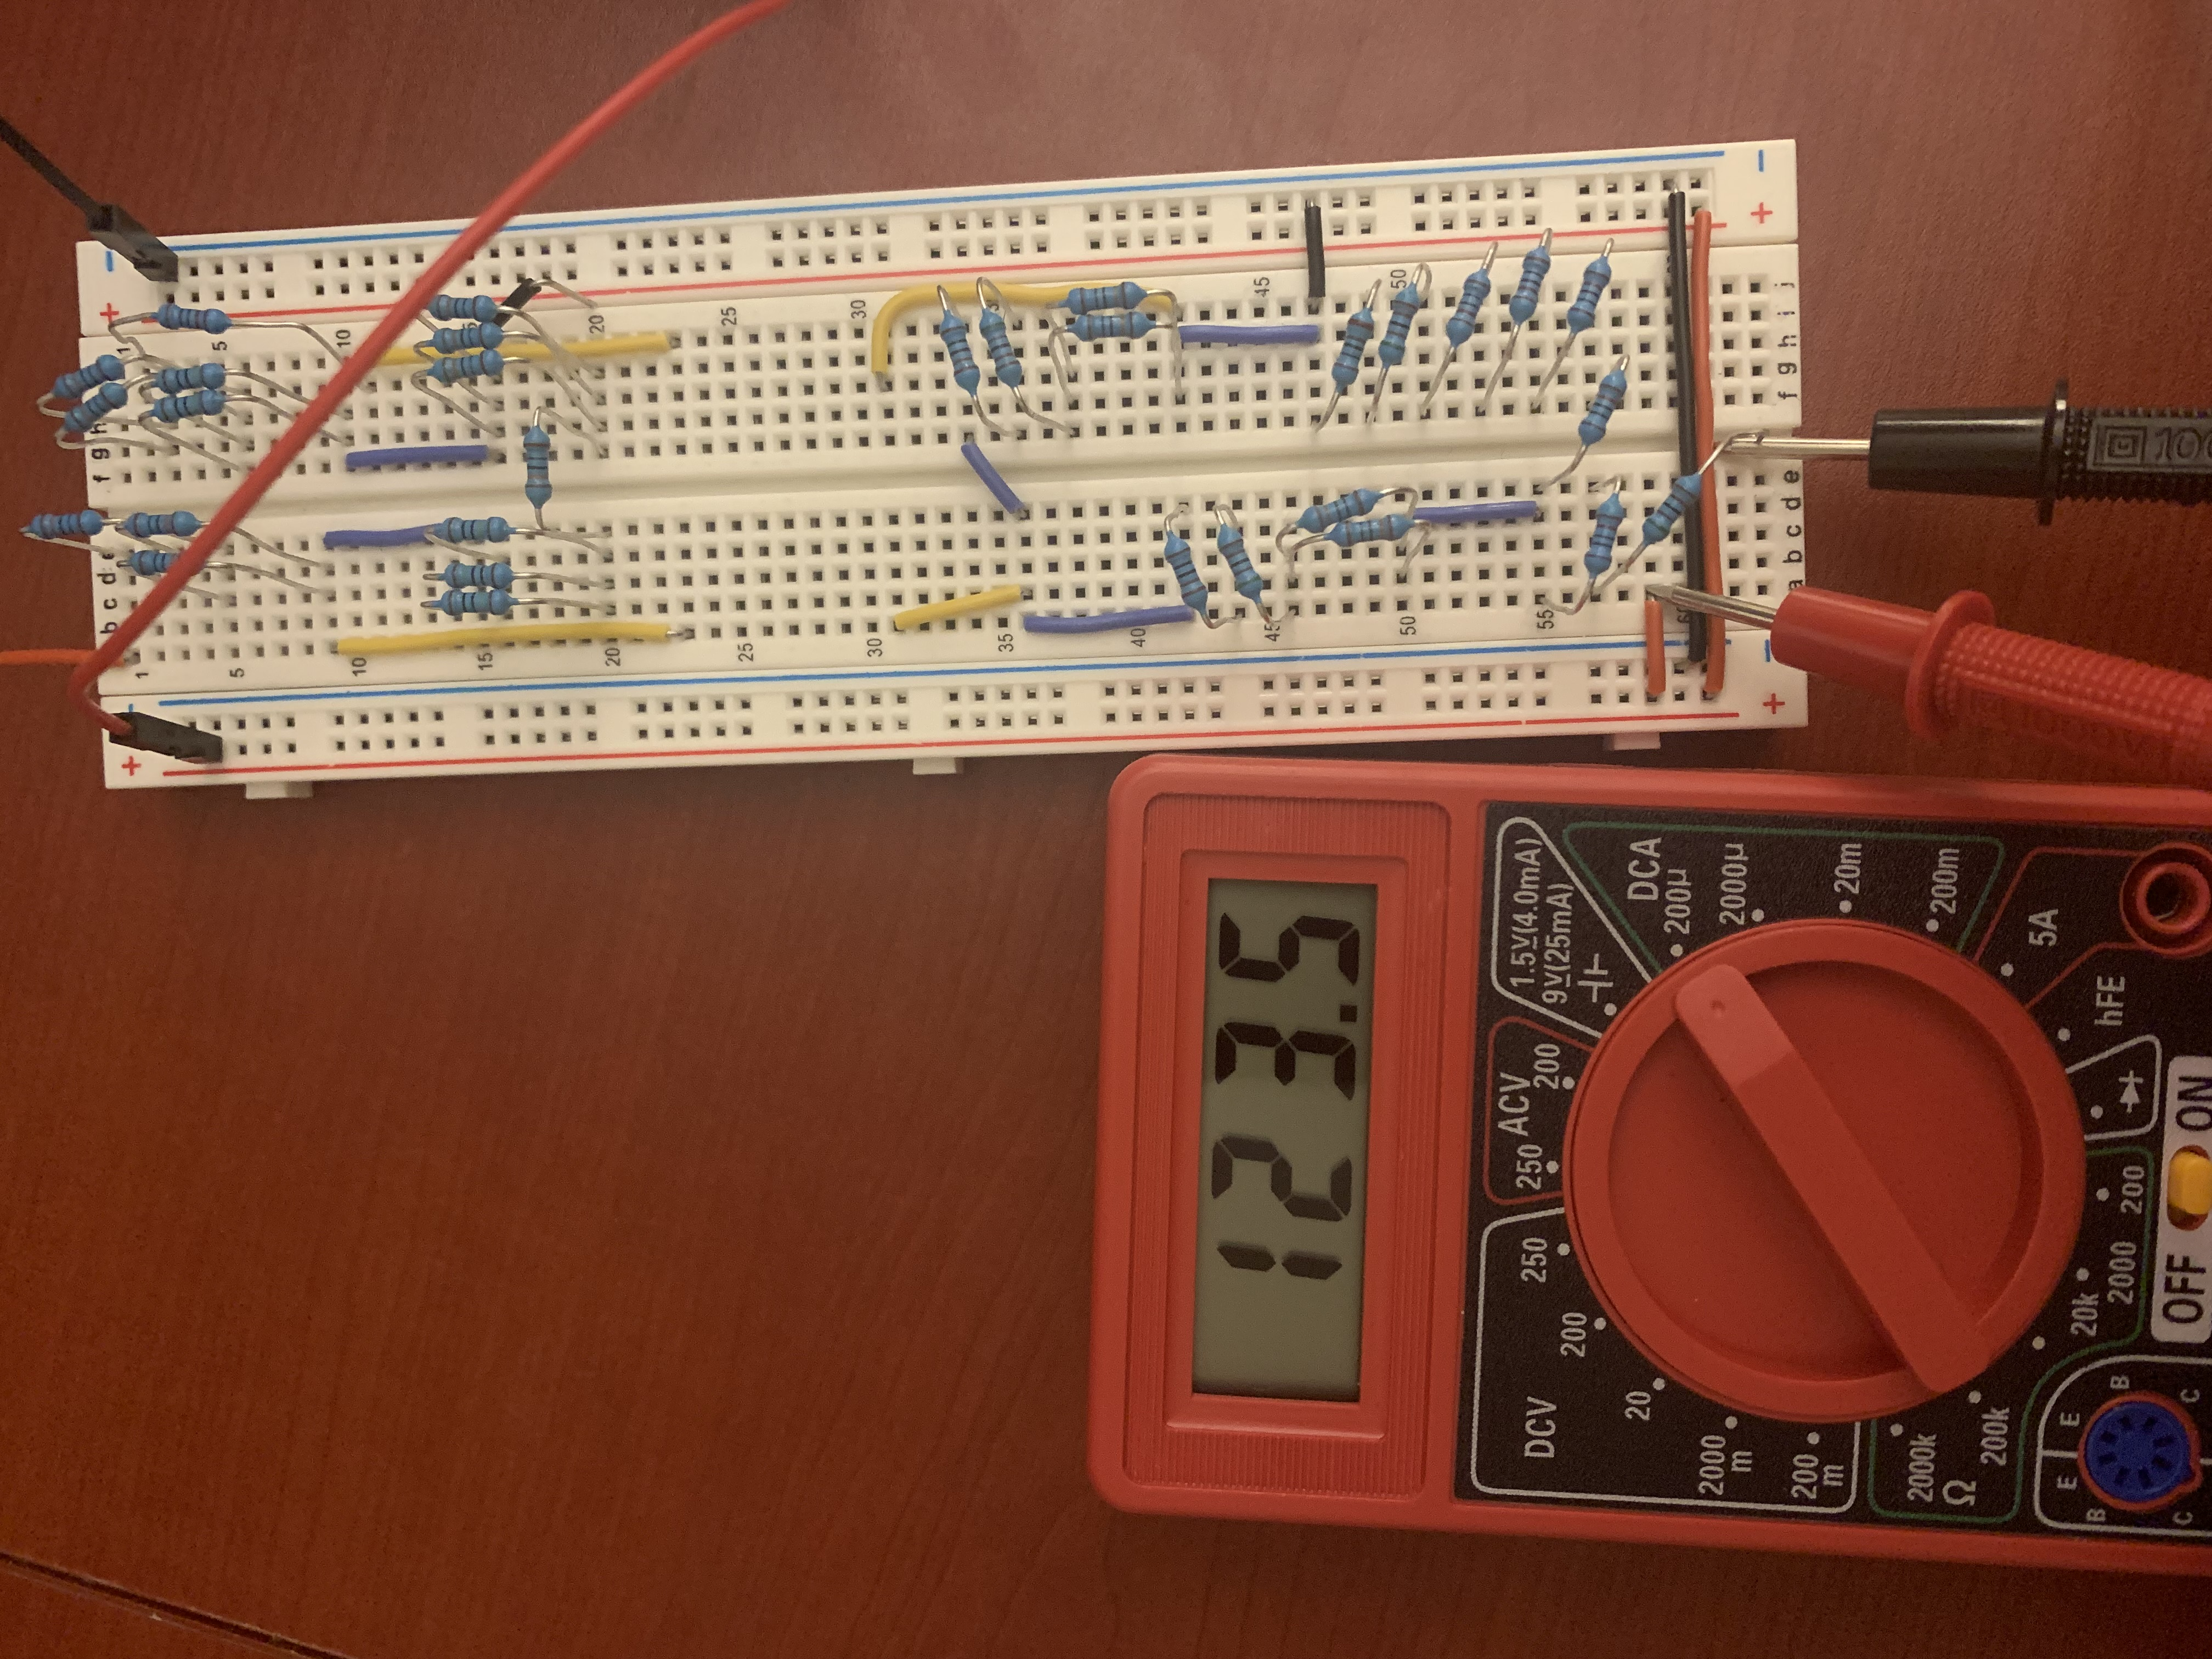
\includegraphics[width=0.8\textwidth]{res/IMG_0151.jpg}
	\newline
	Measuring current
\end{center}

\end{document}
